\input{Configuraciones/paquetes}

%--------------------------

\begin{document}
 \thispagestyle{empty} 
    \begin{tabular}{p{15.5cm}}
    \begin{tabbing}
    \textbf{Universidad del Valle de Guatemala} \\\\
   \textbf{Estudiantes:} Rudik Rompich, Alejandro García Aguirre, Lisandro Toruño\\

    \end{tabbing}
    \begin{center}
        Teoría electromagnética 1 - Catedrático: Eduardo Álvarez\\
        \today
    \end{center}\\
    \hline
    \\
    \end{tabular} 
    \vspace*{0.3cm} 
    \begin{center} 
    {\Large \bf  Simulación
} 
        \vspace{2mm}
    \end{center}
    \vspace{0.4cm}
%--------------------------


\begin{problema}
    Mostrar que la ecuación del plano tangente en $\mathbf{p}=\left(x_{0}, y_{0}, z_{0}\right)$ a una superficie regular $S: f(x, y, z)=0$, con 0 un valor regular de $f$ es
    
    $$f_{x}(\mathbf{p})\left(x-x_{0}\right)+f_{y}(\mathbf{p})\left(y-y_{0}\right)+f_{z}(\mathbf{p})\left(z-z_{0}\right)=0$$
    \begin{sol}
        Sea $f: \mathbb{R}^3 \to \mathbb{R}$ una función continua diferenciable con $0$ un valor regular de $f$ y  $S=\{(x,y,z)\in \mathbb{R}^3| f(x,y,z)=0\}$ una superficie regular. Por definición de plano regular, $$T_\mathbf{p}S =\{\mathbf{v}\in \mathbb{R}^3: \mathbf{v} \text{ es tangente a $S$ en $\mathbf{p}$}\}$$
        
        
        Sea $\mathbf{v}\in T_\mathbf{p}S$   tangente a $S$ en $\mathbf{p}\in S$ en donde $\alpha:(-\varepsilon, \varepsilon)\to S\ni \alpha(0)=\mathbf{p}$ y $\alpha'(0)=\mathbf{v}$.   A probar: \begin{align*}
            T_\mathbf{p}S &= f_{x}(\mathbf{p})\left(x-x_{0}\right)+f_{y}(\mathbf{p})\left(y-y_{0}\right)+f_{z}(\mathbf{p})\left(z-z_{0}\right)\\
            &= \langle\left( f_x(\mathbf{p}), f_y(\mathbf{p}), f_z(\mathbf{p})\right), \left( x-x_0, y-y_0, z-z_0\right)\rangle\\
            &= \langle \nabla f (\mathbf{p}), \left( x-x_0, y-y_0, z-z_0\right)\rangle\\
            &= \langle \nabla f (\mathbf{p}), \mathbf{v}\rangle\\
            &= 0.
        \end{align*}
        Ahora bien, definamos $\alpha(t)=(x(t),y(t),z(t))$ que pasa por el punto $\mathbf{p}$ para $t=0$. De esto, tenemos que: 
        \begin{align*}
            f(\alpha(t)) &= f(x(t),y(t),z(t))\\
            &= 0 \quad \text{(definición de $S$) }
        \end{align*}
        Ahora bien, derivando la expresión anterior, tenemos: 
        \begin{align*}
            \frac{d}{dt}f(\alpha(t)) &= \frac{d}{dt}f(x(t),y(t),z(t))\\
            &= \frac{\partial f(x(t),y(t),z(t))}{\partial x}x'(t)+  \frac{\partial f(x(t),y(t),z(t))}{\partial y}y'(t)
            +  \frac{\partial f(x(t),y(t),z(t))}{\partial z}z'(t)\\
            &= f_x(x,y,z) \cdot x'(t)+f_y(x,y,z)\cdot y'(t)+f_z(x,y,z)\cdot z'(t)\\
            &= \langle \nabla f(x,y,z), \alpha'(t)\rangle\\
            &= 0
        \end{align*}
        Entonces, ahora tenemos el caso particular de $t=0$, tal que: 
        \begin{align*}
           \langle \nabla f(\mathbf{p}), \alpha'(0)\rangle &= 0\\
           \langle \nabla f(\mathbf{p}), \mathbf{v}\rangle &= 0
           \intertext{Entonces, si $\mathbf{v}= (x-x_0,y-y_0,z-z_0)$, tal que: }
           \langle \nabla f(\mathbf{p}), (x-x_0,y-y_0,z-z_0)\rangle &= 0
        \end{align*}
    \end{sol}
    \begin{itemize}
        \item ¿Cómo queda la ecuación del plano tangente en el caso de una superfície regular de la forma $z=f(x, y)$ ?
        \begin{sol}
            Sea $g: \mathbb{R}^3 \to \mathbb{R}$ una función continua diferenciable  $S=\{(x,y,z)\in \mathbb{R}^3| g(x,y,z)=f(x,y)-z\}$ una superficie regular. Ahora bien, notamos que entonces, tenemos un caso particular del inciso anterior, por lo que solo hace falta calcular el gradiente: 
            \begin{align*}
               \langle \nabla g(\mathbf{p}), (x-x_0,y-y_0,z-z_0)\rangle &= 0\\
               \langle \left(g_x(x_0,y_0), g_y(x_0,y_0), g_z(x_0,y_0)\right), (x-x_0,y-y_0,z-z_0)\rangle &= 0\\
               \langle \left(g_x(x_0,y_0), g_y(x_0,y_0), -1\right), (x-x_0,y-y_0,z-z_0)\rangle &= 0\\
               g_x(x_0,y_0)(x-x_0)+g_y(x_0,y_0)(y-y_0)-1(z-z_0) &=0
            \end{align*}
        \end{sol}
    \end{itemize}

\end{problema}

\begin{problema}
    Pruebe que las normales a una superficie parametrizada de la forma

$$
\mathbf{x}(u, v)=(f(u) \cos v, f(u) \sin v, g(u)), \quad f(u) \neq 0, g^{\prime}(u) \neq 0
$$

pasan todas por el eje $O z$

\begin{dem}
    A probar: las normales a una superficie parametrizada de la forma $\mathbf{x}(u, v)=(f(u) \cos v, f(u) \sin v, g(u))$, donde $f(u) \neq 0$ y $g^{\prime}(u) \neq 0$, pasan todas por el eje $O z$. Sea entonces: 
    \begin{itemize}
        \item La forma de los vectores normales. Calculamos las derivadas parciales de $\mathbf{x}$ con respecto a $u$ y $v$:

        $$ \mathbf{x}_u(u,v) = (f’(u)\cos v,f’(u)\sin v,g’(u)) $$
        
        $$ \mathbf{x}_v(u,v) = (-f(u)\sin v,f(u)\cos v,0) $$
        
        Entonces, el vector normal a la superficie en el punto $(u,v)$ está dado por el producto cruz de $\mathbf{x}_u$ y $\mathbf{x}_v$:
        
        
        \begin{align*}
            \mathbf{n}(u,v) &= \mathbf{x}_u \times \mathbf{x}_v\\
            &= \begin{vmatrix} \mathbf{i} & \mathbf{j} & \mathbf{k} \\ f’(u)\cos v & f’(u)\sin v & g’(u) \\ -f(u)\sin v & f(u)\cos v & 0 \end{vmatrix}\\
            &= (-f(u)g’(u)\cos v,-f(u)g’(u)\sin v,f’(u)f(u))
        \end{align*}
        \item Ahora bien, es necesario mostrar que todas las normales pasan por $Oz$. Si trazamos una línea desde un punto $(u,v)$ en la superficie en la dirección del vector normal $\mathbf{n}(u,v)$, tenemos que la ecuación de esta línea es:
        \begin{align*}
            (x,y,z) &= \mathbf{x}(u,v) + t\mathbf{n}(u,v) \\
            &= \begin{pmatrix}f(u)\cos v , f(u)\sin v , g(u)\end{pmatrix} + t\begin{pmatrix}-f(u)g'(u)\cos v , -f(u)g’(u)\sin v , f’(u)f(u)\end{pmatrix}
        \end{align*}
        Ahora bien,  debemos encontrar el punto donde esta línea intersecta al eje $Oz$, por lo que debemos encontrar el valor de $t$ para el cual $x=y=0$. Es decir, tenemos el sistema de ecuaciones: 
        \begin{align*}
            0 &= f(u)\cos v - tf(u)g’(u)\cos v\\
            0 &= f(u)\sin v - tf(u)g’(u)\sin v\\
            z &= g(u) + tf’(u)f(u)
        \end{align*}
        Despejando para $t$ en las primeras dos expresiones, 
        $$t=\frac{1}{g'(u)}$$
        Reemplazando este valor en $z$, tenemos: 
        $$z = g(u) + \frac{f’(u)f(u)}{g'(u)}$$
        Este valor de $z$ no depende de $v$, lo que significa que todas las normales a la superficie pasan por el eje $Oz$.
    \end{itemize}

\end{dem}
\end{problema}

\begin{problema}
    Un punto crítico de una función diferenciable $f: S \rightarrow \mathbb{R}$ definida sobre una superficie regular $S$ es un punto $\mathbf{p}\in S$ tal que $Df(\mathbf{p})=0$
    \begin{enumerate}
        \item Si $f: S \rightarrow \mathbb{R}$ es dada por $f(\mathbf{p})=\left|\mathbf{p}-\mathbf{p}_{0}\right|$, con $\mathbf{p}_{0} \notin S$, mostrar que $\mathbf{p}$ es punto crítico de $f$ si, y sólo si, la recta de $\mathbf{p}$ a $\mathbf{p}_{0}$ es normal a $S$.
        \begin{dem}
            Por definición de plano regular tenemos, $\mathbf{v}\in T_{\mathbf{p}}S$ tangente a $S$ en $\mathbf{p}\in S$ en donde $\alpha: (-\varepsilon, \varepsilon)\rightarrow S$ tal que $\alpha(0)=\mathbf{p}$ y $\alpha’(0)=\mathbf{v}$. A probar: $Df(\mathbf{p})=0 \iff \mathbf{p}-\mathbf{p}_0 \perp T_\mathbf{p} S$. Por otra parte, la derivada de $f$ en el punto $\mathbf{p}$ en la dirección de $\mathbf{v}$ se define como:

$$Df(\alpha(t)) =\frac{d}{dt}f(\alpha(t)),\quad t=0 $$

Además, tenemos por hipótesis que 
\begin{align*}
    f(\mathbf{p})=\left|\mathbf{p}-\mathbf{p}_{0}\right| =\sqrt{\left\langle\mathbf{p}-\mathbf{p}_{0}, \mathbf{p}-\mathbf{p}_{0}\right\rangle}
\end{align*}
 Con esto, podemos calcular su derivada en un punto $\mathbf{p} \in S$ en la dirección de $\mathbf{v}$:

\begin{align*} 
    D f(\alpha(t)) =\frac{d}{dt}f(\alpha(t))&= \frac{d}{dt}\sqrt{\left\langle\alpha(t)-\mathbf{p}_{0}, \alpha(t)-\mathbf{p}_{0}\right\rangle}\\
     &= \frac{1}{2\sqrt{\left\langle\alpha(t)-\mathbf{p}_{0}, \alpha(t)-\mathbf{p}_{0}\right\rangle}}\frac{d}{dt}\left\langle\alpha(t)-\mathbf{p}_{0}, \alpha(t)-\mathbf{p}_{0}\right\rangle \\ 
     &= \frac{1}{2\sqrt{\left\langle\alpha(t)-\mathbf{p}_{0}, \alpha(t)-\mathbf{p}_{0}\right\rangle}}\cdot 2\left\langle\alpha’(t), \alpha(t)-\mathbf{p}_0\right\rangle\\
      &= \frac{\left\langle\alpha’(t), \alpha(t)-\mathbf{p}_0\right\rangle}{\sqrt{\left\langle\alpha(t)-\mathbf{p}_{0}, \alpha(t)-\mathbf{p}_{0}\right\rangle}}\\
      &= \frac{\left\langle\alpha’(t), \alpha(t)-\mathbf{p}_0\right\rangle}{|\alpha(t)-\mathbf{p}_0|}
      \intertext{Cuando $t=0$,}
      Df(\alpha (0))&= \frac{\left\langle\alpha’(0), \alpha(0)-\mathbf{p}_0\right\rangle}{|\alpha(0)-\mathbf{p}_0|}\\
      Df(\mathbf{p})&= \frac{\left\langle\mathbf{v}, \mathbf{p}-\mathbf{p}_0\right\rangle}{|\mathbf{p}-\mathbf{p}_0|}
    \end{align*}
    Con esto, procedemos a probar las dos implicaciones: 
    \begin{itemize}
        \item $(\implies)$ Si $\mathbf{p}$ es un punto crítico de $f\implies Df(\mathbf{p})=0$ entonces: 
        \begin{align*}
            Df(\mathbf{p})&= \frac{\left\langle\mathbf{v}, \mathbf{p}-\mathbf{p}_0\right\rangle}{|\mathbf{p}-\mathbf{p}_0|}=0
        \end{align*}
        Entonces 
        $$\left\langle\mathbf{v}, \mathbf{p}-\mathbf{p}_0\right\rangle =0$$
        Por lo tanto,  la recta de $\mathbf{p}$ a $\mathbf{p}_{0}$ es normal a $S$. 
        \item $(\impliedby)$ Tenemos que la recta de $\mathbf{p}$ a $\mathbf{p}_{0}$ es normal a $S\implies \left\langle\mathbf{v}, \mathbf{p}-\mathbf{p}_0\right\rangle =0\implies Df(\mathbf{p})=0\implies \mathbf{p}$ es un punto crítico de $f$. 
    \end{itemize}
        \end{dem}

        \item Si $h: S \rightarrow \mathbb{R}$ es dada por $h(\mathbf{p})=\mathbf{p} \cdot \mathbf{v}, \mathbf{v} \in \mathbb{R}^{3}$ vector unitario, mostrar que $\mathbf{p}$ es punto crítico de $h$ si, y sólo si, $\mathbf{v}$ es un vector normal a $S$ en $\mathbf{p}$.
        \begin{dem}
            Por definición de plano regular tenemos, $\mathbf{w}\in T_{\mathbf{p}}S$ tangente a $S$ en $\mathbf{p}\in S$ en donde $\alpha: (-\varepsilon, \varepsilon)\rightarrow S$ tal que $\alpha(0)=\mathbf{p}$ y $\alpha’(0)=\mathbf{w}$. A probar: $Dh(\mathbf{p})=0 \iff \langle \mathbf{v}, \mathbf{w} \rangle=0$. Por otra parte, la derivada de $f$ en el punto $\mathbf{p}$ en la dirección de $\mathbf{w}$ se define como:

$$Dh(\alpha(t)) =\frac{d}{dt}h(\alpha(t)),\quad t=0 $$

Además, tenemos por hipótesis que 
\begin{align*}
    h(\mathbf{p})=\mathbf{p}\cdot \mathbf{v}=\langle \mathbf{p}, \mathbf{v} \rangle
\end{align*}
 Con esto, podemos calcular su derivada en un punto $\mathbf{p} \in S$ en la dirección de $\mathbf{v}$:

\begin{align*} 
    D h(\alpha(t)) =\frac{d}{dt}h(\alpha(t))&= \frac{d}{dt} \langle \alpha(t), \mathbf{v} \rangle \\
     &= \langle \alpha'(t), \mathbf{v}\rangle+ \langle \alpha(t),0\rangle\\
     &= \langle \alpha'(t), \mathbf{v}\rangle
      \intertext{Cuando $t=0$,}
      Dh(\alpha (0))&= \langle \alpha'(0), \mathbf{v}\rangle\\
      Dh(\mathbf{p})&= \langle \mathbf{w}, \mathbf{v}\rangle\\
    \end{align*}
    Con esto, procedemos a probar las dos implicaciones: 
    \begin{itemize}
        \item $(\implies)$ Si $\mathbf{p}$ es un punto crítico de $h\implies Dh(\mathbf{p})=0$ entonces: 
        \begin{align*}
            Dh(\mathbf{p})&= \langle \mathbf{w}, \mathbf{v}\rangle=0
        \end{align*}
        
        Por lo tanto,  $\mathbf{v}$ es un vector normal a $S$ en $\mathbf{p}$. 
        \item $(\impliedby)$ Tenemos que $\mathbf{v}$ es un vector normal a $S$ en $\mathbf{p}\implies \left\langle\mathbf{w}, \mathbf{v}\right\rangle =0\implies Dh(\mathbf{p})=0\implies \mathbf{p}$ es un punto crítico de $h$. 
    \end{itemize}
        \end{dem}

        
    \end{enumerate}

\end{problema}

\begin{problema}
    Obtenga la primera forma fundamental de la parametrización de la esfera $S^{2}$ dada por la proyección estereográfica.
    \begin{figure}[H]
        \centering
        \includegraphics[scale=0.5]{imagenes/1.png}
    \end{figure}
    \begin{dem}
        Considerando la tarea anterior, tenemos la proyección estereográfica definida como: 
        $$x(u,v)=\pi^{-1}(u,v) = \left(\frac{4u}{u^2+v^2+4}, \frac{4v}{u^2+v^2+4},\frac{2(u^2+v^2)}{u^2+v^2+4}\right)$$
        Con la siguiente línea de código de \textit{Mathematica} deducimos $x_u$ y $x_v$ respectivamente: 
        \begin{figure}[H]
            \centering
            \includegraphics[scale=0.6]{imagenes/2.png}
        \end{figure}
        \begin{itemize}
            \item $x_u$: 
            $$x_u=\left(\frac{4(4-u^2+v^2)}{(4+u^2+v^2)^2}, -\frac{8uv}{(4+u^2+v^2)^2},\frac{16u}{(4+u^2+v^2)^2}\right)$$
            \item $x_v$: 
            $$x_v=\left(-\frac{8uv}{(4+u^2+v^2)^2},\frac{4(4+u^2-v^2)}{(4+u^2+v^2)^2},\frac{16v}{(4+u^2+v^2)^2}\right)$$
        \end{itemize}

Considerando esto, procedemos a encontrar la primera fórmula fundamental con lo siguiente: 
\begin{align*}
    E = \left\langle x_u,x_u\right\rangle &= \frac{16(4-u^2+v^2)^2}{(4+u^2+v^2)^4}+\frac{64u^2v^2}{(4+u^2+v^2)^4}+\frac{256u^2}{(4+u^2+v^2)^4}\\
    &= \frac{16}{(4+u^2+v^2)^2}\\
     F = \left\langle x_u,x_v\right\rangle &= -\frac{32uv(4-u^2+v^2)}{(4+u^2+v^2)^4}-\frac{32uv(4-u^2+v^2)}{(4+u^2+v^2)^4}+\frac{256uv}{(4+u^2+v^2)^4}\\
     &= 0\\
     G = \left\langle x_v,x_v\right\rangle &= \frac{64u^2v^2}{(4+u^2+v^2)^4}+\frac{16(4+u^2-v^2)^2}{(4+u^2+v^2)^4}+\frac{256v^2}{(4+u^2+v^2)^4}\\
     &= \frac{64u^2v^2+16(4+u^2-v^2)^2+256v^2}{(4+u^2+v^2)^4}\\
     &= \frac{16}{(4+u^2+v^2)^2}
\end{align*}
Por lo tanto, la formula fundamental es: 
\begin{align*}
    I&= \begin{pmatrix}
        u' & v'
    \end{pmatrix}\begin{pmatrix}
        E & F\\
        F & G
    \end{pmatrix} \begin{pmatrix}
        u'\\
        v'
    \end{pmatrix}\\
    &= \begin{pmatrix}
        u' & v'
    \end{pmatrix}\begin{pmatrix}
        \frac{16}{(4+u^2+v^2)^2} & 0\\
        0 &  \frac{16}{(4+u^2+v^2)^2}
    \end{pmatrix} \begin{pmatrix}
        u'\\
        v'
    \end{pmatrix}\\
\end{align*}

    \end{dem}
    
\end{problema}

\begin{problema}
    Muestre que el área $A$ de una región limitada $R$ sobre la superficie $z=f(x, y)$, con $f$ diferenciable, es

$$
A=\iint_{Q} \sqrt{1+f_{x}^{2}+f_{y}^{2}} d x d y
$$

donde $Q$ es la proyección ortogonal de $R$ sobre el plano $O x y$. 
\begin{dem}
    Considérese la siguiente figura: 
        \begin{figure}[H]
            

% Pattern Info
 
\tikzset{
    pattern size/.store in=\mcSize, 
    pattern size = 5pt,
    pattern thickness/.store in=\mcThickness, 
    pattern thickness = 0.3pt,
    pattern radius/.store in=\mcRadius, 
    pattern radius = 1pt}
    \makeatletter
    \pgfutil@ifundefined{pgf@pattern@name@_yxm820imr}{
    \pgfdeclarepatternformonly[\mcThickness,\mcSize]{_yxm820imr}
    {\pgfqpoint{0pt}{0pt}}
    {\pgfpoint{\mcSize}{\mcSize}}
    {\pgfpoint{\mcSize}{\mcSize}}
    {
    \pgfsetcolor{\tikz@pattern@color}
    \pgfsetlinewidth{\mcThickness}
    \pgfpathmoveto{\pgfqpoint{0pt}{\mcSize}}
    \pgfpathlineto{\pgfpoint{\mcSize+\mcThickness}{-\mcThickness}}
    \pgfpathmoveto{\pgfqpoint{0pt}{0pt}}
    \pgfpathlineto{\pgfpoint{\mcSize+\mcThickness}{\mcSize+\mcThickness}}
    \pgfusepath{stroke}
    }}
    \makeatother
    \tikzset{every picture/.style={line width=0.75pt}} %set default line width to 0.75pt        
    
    \begin{tikzpicture}[x=0.75pt,y=0.75pt,yscale=-1,xscale=1]
    %uncomment if require: \path (0,300); %set diagram left start at 0, and has height of 300
    
    %Shape: Polygon Curved [id:ds6892837218684083] 
    \draw  [pattern=_yxm820imr,pattern size=8.55pt,pattern thickness=0.75pt,pattern radius=0pt, pattern color={rgb, 255:red, 0; green, 0; blue, 0}] (323,29.2) .. controls (363,0.2) and (398,12.2) .. (449,14.2) .. controls (500,16.2) and (627,85.2) .. (580,64.2) .. controls (533,43.2) and (410,107.2) .. (431,144.2) .. controls (452,181.2) and (292,108.2) .. (241,121.2) .. controls (190,134.2) and (283,58.2) .. (323,29.2) -- cycle ;
    %Shape: Axis 2D [id:dp18872532511067452] 
    \draw [color={rgb, 255:red, 0; green, 0; blue, 0 }  ,draw opacity=1 ][line width=1.5]  (69.74,268.32) -- (527.41,268.32)(319.84,145.2) -- (92.8,282) (528.71,263.32) -- (527.41,268.32) -- (512.12,273.32) (303.23,152.2) -- (319.84,145.2) -- (313.23,152.2) (170.8,263.32) -- (154.21,273.32)(217.8,263.32) -- (201.21,273.32)(264.8,263.32) -- (248.21,273.32)(311.8,263.32) -- (295.21,273.32)(358.8,263.32) -- (342.21,273.32)(405.8,263.32) -- (389.21,273.32)(452.8,263.32) -- (436.21,273.32)(499.8,263.32) -- (483.21,273.32)(188.51,221.32) -- (198.51,221.32)(266.51,174.32) -- (276.51,174.32) ;
    \draw [color={rgb, 255:red, 255; green, 0; blue, 0 }  ,opacity=1 ]  ;
    %Straight Lines [id:da5156374848971425] 
    \draw [line width=1.5]  [dash pattern={on 5.63pt off 4.5pt}]  (306,96) -- (301,188.2) ;
    %Straight Lines [id:da16859753303957103] 
    \draw [line width=1.5]  [dash pattern={on 5.63pt off 4.5pt}]  (401,124) -- (397,247.2) ;
    %Straight Lines [id:da7013211600122059] 
    \draw [line width=1.5]  [dash pattern={on 5.63pt off 4.5pt}]  (459.65,73.84) -- (456,169.2) ;
    %Straight Lines [id:da7071878519962154] 
    \draw [line width=1.5]  [dash pattern={on 5.63pt off 4.5pt}]  (391.65,47.84) -- (384,169.2) ;
    %Shape: Regular Polygon [id:dp9111656039106069] 
    \draw  [color={rgb, 255:red, 45; green, 49; blue, 92 }  ,draw opacity=0.48 ][fill={rgb, 255:red, 27; green, 24; blue, 24 }  ,fill opacity=0.76 ][line width=1.5]  (344.85,64.38) .. controls (382.92,47.34) and (377.72,50.75) .. (400.05,49.17) .. controls (422.38,47.59) and (479.51,86.89) .. (459.05,78.98) .. controls (438.59,71.07) and (390.53,103.92) .. (401,124) .. controls (411.47,144.08) and (329.62,107.57) .. (312.97,107.57) .. controls (296.31,107.57) and (306.78,81.41) .. (344.85,64.38) -- cycle ;
    %Shape: Polygon Curved [id:ds6344597551586724] 
    \draw  [fill={rgb, 255:red, 0; green, 0; blue, 0 }  ,fill opacity=0.14 ][dash pattern={on 5.63pt off 4.5pt}][line width=1.5]  (327,178.2) .. controls (347,168.2) and (487,152.2) .. (448,181) .. controls (409,209.8) and (389,203.2) .. (409,233.2) .. controls (429,263.2) and (301,246.2) .. (281,216.2) .. controls (261,186.2) and (307,188.2) .. (327,178.2) -- cycle ;
    
    % Text Node
    \draw (544,257.4) node [anchor=north west][inner sep=0.75pt]    {$x$};
    % Text Node
    \draw (283,137.4) node [anchor=north west][inner sep=0.75pt]    {$y$};
    % Text Node
    \draw (379.16,63.4) node [anchor=north west][inner sep=0.75pt]  [font=\Large,color={rgb, 255:red, 255; green, 0; blue, 0 }  ,opacity=1 ,xslant=0.54]  {$R$};
    % Text Node
    \draw (203,38.4) node [anchor=north west][inner sep=0.75pt]    {$z=( x,y)$};
    % Text Node
    \draw (354.16,182.4) node [anchor=north west][inner sep=0.75pt]  [font=\Large,color={rgb, 255:red, 255; green, 0; blue, 0 }  ,opacity=1 ,xslant=0.54]  {$Q$};
    
    
    \end{tikzpicture}
        \end{figure}
        Por el siguiente teorema deducido en clase: 
        \begin{cajita}
            Sea $S\subset \mathbb{R}^3$ una superficie regular y $R\subseteq S$ una región limitada en $S$, contenida dentro de una vecindad parametrizada $\mathbf{x}:U\subseteq \mathbb{R}^2\to S$. Entonces, el área superficial de $R$ está dada por 
            $$A(R)=\int\int_Q |\mathbf{x}_u\times \mathbf{x}_v|dudv, \quad Q=\mathbf{x}^{-1}(R)$$
        \end{cajita}
        Por la hipótesis, tenemos $\mathbf{x}:U\subseteq\mathbb{R}^2\to S$ tal que 
        $$\mathbf{x}(x,y)=(x,y,f(x,y)),$$
        tal que el área superficial (donde $Q$ es la proyección ortogonal de $R$, es decir $\pi(x,y,z)=(x,y)$): 
        $$A(R)=\int\int_Q |\mathbf{x}_x\times \mathbf{x}_y|dxdy, \quad Q=\mathbf{x}^{-1}(R)=\pi(R)$$
        Entonces, tenemos: 
        $$\mathbf{x}_x = \left(1,0,f_x\right) \quad \mathbf{x}_y = \left(0,1,f_y\right)$$
        Tal que: 
        \begin{align*}
            \mathbf{x}_x \times \mathbf{x}_y = \begin{vmatrix} \mathbf{i} & \mathbf{j} & \mathbf{k} \\
                 1 & 0 & f_x \\
                  0 & 1 & f_y \end{vmatrix} = \left(-f_x, -f_y, 1\right)
        \end{align*}
        Por lo tanto, 
        \begin{align*}
            A(R)&=\int\int_Q |\mathbf{x}_x\times \mathbf{x}_y|dxdy\\
            &= \int\int_Q |\left(-f_x, -f_y, 1\right)|dxdy\\
            &= \iint_{Q} \sqrt{1+f_{x}^{2}+f_{y}^{2}} d x d y
        \end{align*}
\end{dem}

\end{problema}

\begin{problema}
    Las curvas coordenadas de una parametrización $\mathbf{x}(u, v)$ de $S$ constituyen una red de Tchebyshev si las longitudes de los lados opuestos de cualquier cuadrilátero formado por ellas son iguales.

    \begin{enumerate}
        \item Pruebe una condición necesaria y sufieciente para que esto suceda es que

        $$
        \frac{\partial E}{\partial v}=0 \quad \text { y } \quad \frac{\partial G}{\partial u}=0
        $$
        \begin{dem}
            A probar: las curvas coordenadas de una parametrización $\mathbf{x}(u, v)$ de $S$ constituyen una red de Tchebyshev si las longitudes de los lados opuestos de cualquier cuadrilátero formado por ellas son iguales. $\iff \frac{\partial E}{\partial v}=0 \wedge \frac{\partial G}{\partial u}=0$.

Considérese la primera forma fundamental de una superficie se define como:

$$I= \begin{pmatrix}
    u' & v'
\end{pmatrix}\begin{pmatrix}
    E & F\\
    F & G
\end{pmatrix} \begin{pmatrix}
    u'\\
    v'
\end{pmatrix}$$


En donde $E = \langle \mathbf{x}_u,\mathbf{x}_u \rangle$, $F = \langle \mathbf{x}_u,\mathbf{x}_v \rangle$ y $G = \langle \mathbf{x}_v,\mathbf{x}_v \rangle$. Ahora bien, consideremos un cuadrilátero formado por las curvas coordenadas de la parametrización $\mathbf{x}(u, v)$ en la superficie $S$, formado por los vértices del cuadrilátero son $\mathbf{x}(u_0,v_0)$, $\mathbf{x}(u_0,v_1)$, $\mathbf{x}(u_1,v_0)$ y $\mathbf{x}(u_1,v_1)$, considérese la siguiente ilustración:

\begin{figure}[H]
    \centering
    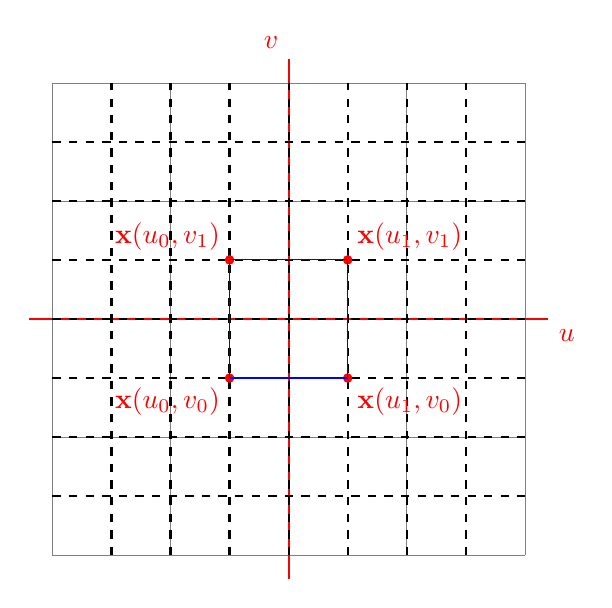
\begin{tikzpicture}[scale=1.5]
        \draw[step=1cm,gray,very thin] (-2,-2) grid (2,2);
        \draw[thick,red] (-2.2,0) -- (2.2,0) node[anchor=north west] {$u$};
        \draw[thick,red] (0,-2.2) -- (0,2.2) node[anchor=south east] {$v$};
        
        \foreach \x in {-1.5,-1,...,1.5} {
            \draw[dashed, thick] (\x,-2) -- (\x,2);
        }
        
        \foreach \y in {-1.5,-1,...,1.5} {
            \draw[dashed,thick] (-2,\y) -- (2,\y);
        }
        
        \coordinate (A) at (-0.5,-0.5);
        \coordinate (B) at (-0.5,0.5);
        \coordinate (C) at (0.5,-0.5);
        \coordinate (D) at (0.5,0.5);
        
        \filldraw[red] (A) circle (1pt) node[anchor=north east] {$\mathbf{x}(u_0,v_0)$};
        \filldraw[red] (B) circle (1pt) node[anchor=south east] {$\mathbf{x}(u_0,v_1)$};
        \filldraw[red] (C) circle (1pt) node[anchor=north west] {$\mathbf{x}(u_1,v_0)$};
        \filldraw[red] (D) circle (1pt) node[anchor=south west] {$\mathbf{x}(u_1,v_1)$};
        
        \draw[blue] (A) -- (B);
        \draw[blue] (C) -- (D);
        \draw[blue] (A) -- (C);
        \draw[blue] (B) -- (D);
        
        
        \end{tikzpicture}
\end{figure}

Ahora bien, la longitud de la curva, de acuerdo a la definición vista en clase: 

\begin{cajita}
    Dado $\mathbf{x}(u(t),v(t))$ con $t$ en el intervalo $[a,b]$, entonces la longitud de la curva está dada por:

$$ L(\alpha(t)) = \int_a^b \sqrt{E\left(\frac{du}{dt}\right)^2 + 2F\left(\frac{du}{dt}\right)\left(\frac{dv}{dt}\right) +G\left(\frac{dv}{dt}\right)^2}dt $$
\end{cajita}

Ahora bien, calculamos las longitudes de los lados opuestos: 
\begin{itemize}
    \item La longitud del lado opuesto al lado formado por los puntos $\mathbf{x}(u_0,v_0)$ y $\mathbf{x}(u_0,v_1)$. Consideremos el segmento de curva en la superficie que une los puntos $\mathbf{x}(u_1,v_0)$ y $\mathbf{x}(u_1,v_1)$. Este segmento de curva puede ser parametrizado por $\mathbf{x}(u_1,v)$ con $v$ en el intervalo $[v_0,v_1]$. Entonces tenemos: 
    

    \begin{align*} |\mathbf{x}(u_1,v_0) - \mathbf{x}(u_1,v_1)| &= |L(\mathbf{x}(u_1,v))|\\
        &= \left|\int_{v_0}^{v_1} \sqrt{E\left(\frac{du}{dv}\right)^2 + 2F\frac{du}{dv}\frac{dv}{dv} + G\left(\frac{dv}{dv}\right)^2}dv\right|\\
        &= \left|\int_{v_0}^{v_1} \sqrt{E\left(0\right)^2 + 2F(0)(1) + G\left(1\right)^2}dv\right|\\
        &= \left|\int_{v_0}^{v_1} \sqrt{G(u_1,v)}dv\right|
    \end{align*}
    \item 

    La longitud del lado opuesto al lado formado por los puntos $\mathbf{x}(u_0,v_0)$ y $\mathbf{x}(u_1,v_0)$.  Consideremos el segmento de curva en la superficie que une los puntos $\mathbf{x}(u_0,v_1)$ y $\mathbf{x}(u_1,v_1)$. Este segmento de curva puede ser parametrizado por $\mathbf{x}(u,v_1)$ con $u$ en el intervalo $[u_0,u_1]$. Entonces tenemos: 
    

    \begin{align*}|\mathbf{x}(u_0,v_1) - \mathbf{x}(u_1,v_1)| &= |L(\mathbf{x}(u,v_1))|\\
        &= \left|\int_a^b \sqrt{E\left(\frac{du}{du}\right)^2 + 2F\left(\frac{du}{du}\right)\left(\frac{dv}{du}\right) +G\left(\frac{dv}{du}\right)^2}dt\right|\\
        &= \left|\int_a^b \sqrt{E\left(1\right)^2 + 2F\left(1\right)\left(0\right) +G\left(0\right)^2}dt\right|\\
        &= \left|\int_a^b \sqrt{E(u,v_1)}dt\right|
    \end{align*}
\end{itemize}

Entonces, lo que la hipótesis nos dice es que los lados opuestos del cuadrilátero sean iguales, es decir:

$$ \int_{v_0}^{v_1} \sqrt{G(u_1,v)}dv = \int_{u_0}^{u_1} \sqrt{E(u,v_1)}du $$. 
Entonces, procedemos por doble implicación: 

\begin{itemize}
    \item $(\implies)$  Las curvas coordenadas de una parametrización $\mathbf{x}(u, v)$ de $S$ constituyen una red de Tchebyshev si las longitudes de los lados opuestos de cualquier cuadrilátero formado por ellas son iguales $\implies$ 
    $$ \int_{v_0}^{v_1} \sqrt{G(u_1,v)}dv = \int_{u_0}^{u_1} \sqrt{E(u,v_1)}du $$
    Ambas expresiones son constantes, entonces si las derivamos 

    $$ \frac{\partial}{\partial u}\left(\int_{v_0}^{v_1} \sqrt{G(u_1,v)}dv\right) = 0 \implies \int_{v_0}^{v_1} \frac{\partial}{\partial u}\sqrt{G(u_1,v)}dv = 0 \implies \frac{\partial}{\partial u}\sqrt{G(u_1,v)} = 0 $$


$$ \frac{\partial}{\partial v}\left(\int_{u_0}^{u_1} \sqrt{E(u,v_1)}du\right) = 0 \implies  \int_{u_0}^{u_1} \frac{\partial}{\partial v}\sqrt{E(u,v_1)}du = 0 \implies  \frac{\partial}{\partial v}\sqrt{E(u,v_1)} = 0$$

Por lo tanto, 
$$
        \frac{\partial E}{\partial v}=0 \quad \text { y } \quad \frac{\partial G}{\partial u}=0.
        $$

    \item $(\impliedby)$ Ahora, sea 
    $$
        \frac{\partial E}{\partial v}=0 \quad \text { y } \quad \frac{\partial G}{\partial u}=0.
        $$

    Entonces, si integramos ambas expresiones tenemos: 
    $$
        E=E(v) \quad \text { y } \quad G=G(u).
        $$

    y el procedimiento es el mismo que en la condición anterior, solo que yendo de regreso. 
\end{itemize}


\end{dem}
        
        \item Mostrar que si las curvas coordenadas forman una red de Tchebyshev, entonces es posible reparametrizar la vecindad coordenada de tal forma que $E=1, F=\cos \theta$ y $G=1$.
        \begin{dem} Supongamos que las curvas coordenadas de una parametrización $\mathbf{x}(u, v)$ de una superficie $S$ forman una red de Tchebyshev y considérese lo deducido en el inciso anterior. Entonces, lo que nos están pidiendo son funciones $f(u,v)$ y $g(u,v)$ tales que $\mathbf{x}(u,v) = \mathbf{x}(f(u,v),g(u,v))$, tal que si elegimos $f$ y $g$ adecuadamente, podemos hacer que los coeficientes $E$, $F$ y $G$, sean: 
            \begin{align*}
                E &= \left\langle \frac{\partial \mathbf{x}}{\partial f}, \frac{\partial \mathbf{x}}{\partial f} \right\rangle = 1\\
                 F &= \left\langle \frac{\partial \mathbf{x}}{\partial f}, \frac{\partial \mathbf{x}}{\partial g} \right\rangle =\cos \theta \\
             G &= \left\langle \frac{\partial \mathbf{x}}{\partial g}, \frac{\partial \mathbf{x}}{\partial g} \right\rangle =1
            \end{align*}
            Además, tenemos: 
            $$ \int_{v_0}^{v_1} \sqrt{G(u_1,v)}dv = \int_{u_0}^{u_1} \sqrt{E(u,v_1)}du $$
            Que implica: 
            $$
        \frac{\partial E}{\partial v}=0 \quad \text { y } \quad \frac{\partial G}{\partial u}=0.
        $$
            De esto, elegimos arbitrariamente que: 
            \begin{align*}
                f(u,v) &=  \int_{v_0}^{v_1} \sqrt{G(u_1,v)}dv \\
                g(u,v) &= \int_{u_0}^{u_1} \sqrt{E(u,v_1)}du
            \end{align*}
            Entonces, procedemos a encontrar las derivadas de $\mathbf{x}(u,v)$:
            \begin{align*}
                \frac{\partial \mathbf{x}}{\partial u} &= \frac{\partial \mathbf{x}}{\partial f} \frac{\partial f}{\partial u} + \frac{\partial \mathbf{x}}{\partial g} \frac{\partial g}{\partial u}\\
                &= \frac{\partial \mathbf{x}}{\partial f} \left(0\right) + \frac{\partial \mathbf{x}}{\partial g} \left(\sqrt{E(u,v_1)}\right)\\
                &= \frac{\partial \mathbf{x}}{\partial g} \sqrt{E(u,v_1)}
            \end{align*}

            \begin{align*}
                \frac{\partial \mathbf{x}}{\partial v} &= \frac{\partial \mathbf{x}}{\partial f} \frac{\partial f}{\partial v} + \frac{\partial \mathbf{x}}{\partial g} \frac{\partial g}{\partial v}\\
                &= \frac{\partial \mathbf{x}}{\partial f} \left(\sqrt{G(u_1,v)}\right)  + \frac{\partial \mathbf{x}}{\partial g} \left(0\right)\\
                &= \frac{\partial \mathbf{x}}{\partial f} \sqrt{G(u_1,v)} 
            \end{align*}
            Entonces, tenemos que: 
            \begin{align*}
                E &= \left\langle \frac{\partial \mathbf{x}}{\partial f}, \frac{\partial \mathbf{x}}{\partial f} \right\rangle = \left\langle   \frac{\frac{\partial \mathbf{x}}{\partial v}}{\sqrt{G(u_1,v)}},\frac{\frac{\partial \mathbf{x}}{\partial v}}{\sqrt{G(u_1,v)}}\right\rangle  =  \cos 0 =1\\
                 F &= \left\langle \frac{\partial \mathbf{x}}{\partial f}, \frac{\partial \mathbf{x}}{\partial g} \right\rangle = \left\langle   \frac{\frac{\partial \mathbf{x}}{\partial v}}{\sqrt{G(u_1,v)}},\frac{\frac{\partial \mathbf{x}}{\partial u}}{\sqrt{E(u_1,v)}}\right\rangle  =\cos \theta \\
             G &= \left\langle \frac{\partial \mathbf{x}}{\partial g}, \frac{\partial \mathbf{x}}{\partial g} \right\rangle = \left\langle \frac{\frac{\partial \mathbf{x}}{\partial u}}{\sqrt{E(u_1,v)}}, \frac{\frac{\partial \mathbf{x}}{\partial u}}{\sqrt{E(u_1,v)}} \right\rangle  =\cos 0 = 1
            \end{align*}
        \end{dem}
    \end{enumerate}


\end{problema}

\begin{problema}
    Sea $S$ una superficie de revolución y $C: I \rightarrow \mathbb{R}^{2}$ su curva generatriz (en el plano $O x z$ ). Sea $s$ la longitud de arco de la curva, y denotamos por $\rho=\rho(s)$ la distancia del punto correspondiente $C(s)$ al eje de rotación.
    \begin{itemize}
        \item Mostrar el Teorema de Pappus: El área de $S$ está dada por

        $$
        A=2 \pi \int_{0}^{L} \rho(s) d s
        $$
        
        donde $L$ es la longitud de la curva $C$.
        \begin{dem}
            Ya en clase se había deducido la parametrización para una superficie de revolución, Sea $$x=f(v),\quad z=g(v),\quad a<v<b, \quad f(v)>0$$
            la parametrización de $C$. Entonces la parametrización de $S$: 
            $$\mathbf{x}(u,v)=(f(v)\cos u, f(v)\sin u, g(v)), \quad u,v\in (0,2\pi)$$
            Entonces: 
            \begin{align*}
                \mathbf{x}_u &=\left(-f(v)\sin u, f(v)\cos u, 0\right)\\
                \mathbf{x}_v &=\left(f'(v)\cos u, f'(v)\sin u, g'(v)\right)\\
            \end{align*}
            De esto: 
            \begin{align*}
                E &= \langle \mathbf{x}_u, \mathbf{x}_u \rangle = f^2(v)\\
                F &= \langle \mathbf{x}_u, \mathbf{x}_v \rangle = 0\\
                G &= \langle \mathbf{x}_v, \mathbf{x}_v \rangle = f'(v)^2+ g'(v)^2 =1
            \end{align*}
            y 
            \begin{align*}
                A(S) &= \int_0^L \int_0^{2\pi} \sqrt{EG -F^2}du dv\\
                &=\int_0^L \int_0^{2\pi} \sqrt{f^2(v)}du dv\\
                &=\int_0^L \int_0^{2\pi} f(v)du dv\\
                &=2\pi\int_0^L f(v) dv\\
                &= 2\pi\int_0^L \rho(s) ds\\
            \end{align*}
        \end{dem}
        \item Aplicar la parte (a) para calcular el área de la superficie de un toro.
        \begin{dem}
            Este problema se resolvió en clase, en el ejemplo 2 de la presentación de áreas en superficies: 

            \begin{figure}[H]
                \centering
                \includegraphics[scale=0.3]{imagenes/3.png}
            \end{figure}
        \end{dem}
    \end{itemize}

\end{problema}

\begin{problema}
    El gradiente de una función diferenciable $f: S \rightarrow \mathbb{R}$ definida sobre una superficie regular $S \subset \mathbb{R}^{3}$ es la aplicación diferenciable $\nabla f: S \rightarrow \mathbb{R}^{3}$ que asocia a cada punto $\mathbf{p} \in S$ un vector $\nabla f(\mathbf{p}) \in T_{\mathbf{p}} S$ tal que

$$
\langle\nabla f(\mathbf{p}), \mathbf{v}\rangle_{\mathbf{p}}=D f(\mathbf{p}) \cdot \mathbf{v}, \quad \forall \mathbf{v} \in T_{\mathbf{p}} S
$$

Demuestre que si $E, F, G$ son los coeficientes de la primera forma fundamental en una parametrización $\mathbf{x}: U \subseteq \mathbb{R}^{2} \rightarrow S$, entonces el gradiente $\nabla f(\mathbf{p})$ en $\mathbf{x}(U)$ está dado por

$$
\nabla f=\frac{f_{u} G-f_{v} F}{E G-F^{2}} \mathbf{x}_{u}+\frac{f_{v} E-f_{u} F}{E G-F^{2}} \mathbf{x}_{v}
$$

En particular, si $S=\mathbb{R}^{2}$, con coordenadas $x, y$, entonces

$$
\nabla f=f_{x} \mathbf{e}_{1}+f_{y} \mathbf{e}_{2}
$$



\begin{dem} A probar: 
    $$
\nabla f=\frac{f_{u} G-f_{v} F}{E G-F^{2}} \mathbf{x}_{u}+\frac{f_{v} E-f_{u} F}{E G-F^{2}} \mathbf{x}_{v}.
$$
    Sea $\mathbf{x}: U \subseteq \mathbb{R}^{2} \rightarrow S$ una parametrización de la superficie $S$, entonces los coeficientes de la primera forma fundamental son:

$$ E=\left\langle\frac{\partial \mathbf{x}}{\partial u}, \frac{\partial \mathbf{x}}{\partial u}\right\rangle, F=\left\langle\frac{\partial \mathbf{x}}{\partial u}, \frac{\partial \mathbf{x}}{\partial v}\right\rangle, G=\left\langle\frac{\partial \mathbf{x}}{\partial v}, \frac{\partial \mathbf{x}}{\partial v}\right\rangle. $$

Ahora bien, considérese la función $f: S \rightarrow \mathbb{R}$ y su composición con la parametrización $\mathbf{x}: U \subseteq \mathbb{R}^{2} \rightarrow S$ definida como  $f(\mathbf{x}(u,v))$. Obtenemos sus derivadas parciales: 
\begin{align*}
    f_u &= \frac{\partial}{\partial u}f(\mathbf{x}(u,v)) = Df(\mathbf{x}(u,v))\cdot\frac{\partial\mathbf{x}}{\partial u}\\
    f_v &= \frac{\partial}{\partial v}f(\mathbf{x}(u,v)) = Df(\mathbf{x}(u,v))\cdot\frac{\partial\mathbf{x}}{\partial v} 
\end{align*}
Entonces, tenemos la siguiente definición que nos da el problema: 
\begin{cajita}
    El gradiente de una función diferenciable $f: S \rightarrow \mathbb{R}$ definida sobre una superficie regular $S \subset \mathbb{R}^{3}$ es la aplicación diferenciable $\nabla f: S \rightarrow \mathbb{R}^{3}$ que asocia a cada punto $\mathbf{p} \in S$ un vector $\nabla f(\mathbf{p}) \in T_{\mathbf{p}} S$ tal que

$$
\langle\nabla f(\mathbf{p}), \mathbf{v}\rangle_{\mathbf{p}}=D f(\mathbf{p}) \cdot \mathbf{v}, \quad \forall \mathbf{v} \in T_{\mathbf{p}} S
$$
\end{cajita}


Sea $\mathbf{v} = a\frac{\partial\mathbf{x}}{\partial u} + b\frac{\partial\mathbf{x}}{\partial v} \in T_{\mathbf{p}}S$, tenemos que:
\begin{align*}
    Df(\mathbf{x}(u,v))\cdot\mathbf{v} &= Df(\mathbf{x}(u,v))\cdot\left(a\frac{\partial\mathbf{x}}{\partial u} + b\frac{\partial\mathbf{x}}{\partial v}\right)\\
    &= aDf(\mathbf{x}(u,v))\frac{\partial\mathbf{x}}{\partial u} + bDf(\mathbf{x}(u,v))\frac{\partial\mathbf{x}}{\partial v}\\
    &= af_u + bf_v 
\end{align*}



Por otra parte, tenemos el vector $\nabla f = A\frac{\partial\mathbf{x}}{\partial u} + B\frac{\partial\mathbf{x}}{\partial v}$, tal que:

\begin{align*}
    \langle\nabla f,\mathbf{v}\rangle_{\mathbf{p}} &= \left\langle A\frac{\partial\mathbf{x}}{\partial u} + B\frac{\partial\mathbf{x}}{\partial v},a\frac{\partial\mathbf{x}}{\partial u} + b\frac{\partial\mathbf{x}}{\partial v}\right\rangle\\
    &=Aa\left\langle\frac{\partial\mathbf{x}}{\partial u},\frac{\partial\mathbf{x}}{\partial u}\right\rangle
    +Ab\left\langle\frac{\partial\mathbf{x}}{\partial u},\frac{\partial\mathbf{x}}{\partial v}\right\rangle
    +Ba\left\langle\frac{\partial\mathbf{x}}{\partial v},\frac{\partial\mathbf{x}}{\partial u}\right\rangle
    + Bb\left\langle\frac{\partial\mathbf{x}}{\partial v},\frac{\partial\mathbf{x}}{\partial v}\right\rangle \\
    &=AaE+AbF+BaF+ BbG\\
    &= a(AE+ BF)+b(AF+BG)
\end{align*}

Entonces, igualadas ambas expresiones que obtuvimos anteriormente: 
\begin{align*}
\langle\nabla f(\mathbf{p}), \mathbf{v}\rangle_{\mathbf{p}}&=D f(\mathbf{p}) \cdot \mathbf{v}\\
af_u + bf_v &= a(AE+ BF)+b(AF+BG)
\end{align*}
Entonces: 
\begin{align*}
    f_u &= AE+BF\\
    f_v &= AF+BG
\end{align*}

Resolviendo este sistema de ecuaciones para $A$ y $B$,

\begin{figure}[H]
    \centering
    \includegraphics[scale=0.5]{imagenes/4.png}
\end{figure}

Obtenemos que:

$$ A = \frac{f_uG - f_vF}{EG - F^2}\qquad  B = \frac{f_vE - f_uF}{EG - F^2}$$


Por lo tanto, el gradiente $\nabla f$ en $\mathbf{x}(U)$ está dado por:

$$ \nabla f=\frac{f_{u} G-f_{v} F}{E G-F^{2}} \mathbf{x}_{u}+\frac{f_{v} E-f_{u} F}{E G-F^{2}} \mathbf{x}_{v} $$


------------------------------------------------------------------------------------------------------------

Ahora, para el caso particular, si $S=\mathbb{R}^{2}$, con coordenadas $x, y$. A probar:

$$
\nabla f=f_{x} \mathbf{e}_{1}+f_{y} \mathbf{e}_{2}
$$
Entonces, sea 
$$\mathbf{x}(x,y)=(x,y,0)$$
Con sus derivadas: 
\begin{align*}
    \mathbf{x}_x &=(1,0,0) \\
    \mathbf{x}_y &= (0,1,0)\\
\end{align*}
Además: 
$$E=\langle\mathbf{x}_x,\mathbf{x}_x\rangle= 1, \quad F=\langle\mathbf{x}_x,\mathbf{x}_y\rangle= 0, G=\langle\mathbf{x}_y,\mathbf{x}_y\rangle= 1 $$

Por lo tanto,
\begin{align*}
    \nabla f(x,y) &= \frac{f_{x} G-f_{y} F}{E G-F^{2}} \mathbf{x}_{x}+\frac{f_{x} E-f_{y} F}{E G-F^{2}} \mathbf{x}_{y}\\
    &= \frac{f_{x} (1)-f_{y} (0)}{(1) (1)-(0)^{2}} \mathbf{x}_{x}+\frac{f_{x} (1)-f_{y} (0)}{(1) (1)-(0)^{2}} \mathbf{x}_{y}\\
    &= f_{x} \mathbf{x}_{x}+f_{x}\mathbf{x}_{y}\\
    &= f_{x} (1,0,0)+f_{x}(0,1,0)\\
    &= f_{x} \mathbf{e}_{1}+f_{y} \mathbf{e}_{2}
\end{align*}
\end{dem}

\end{problema}

\begin{problema}
    La orientación puede no ser preservada por difeomorfismos.

Sea $\varphi: S_{1} \rightarrow S_{2}$ un difeomorfismo entre superficies.

\begin{enumerate}
    \item Muestre que $S_{1}$ es orientable si y solo si, $S_{2}$ es orientable.
    \begin{dem}
        Tenemos una doble implicación. Considérese las siguientes definiciones vistas en clase: 
        \begin{cajita}
            Una superficie $S\subseteq \mathbf{R}^3$ es orientable cuando existe al menos un atlas coherente de clase $C^k$ en $S$. 
        \end{cajita}
        \begin{cajita}
            Sea $S\subseteq \mathbb{R}^3$ superficie regular. Dos parametrizaciones $x_1:U_1\subseteq \mathbb{R}^2\to V_1\cap S$ y $x_2:U_2\subseteq \mathbb{R}^2\to V_2\cap S$ en la superficie $S$ son \textbf{coherentes} cuando $W=V_1\cap V_2\cap S=\varnothing$, o cuando $W=V_1\cap V_2\cap S\neq \varnothing$ y la matriz jacobiana satisface $\det D(x_2^{-1}\circ x_1)(q)>0,\forall q\in x_1^{-1}(W)$
        \end{cajita}

        Procedemos por doble implicación, la idea de la prueba será demotrar:  $S$ es orientable $\iff$  Una superficie $S\subseteq \mathbf{R}^3$ es orientable cuando existe al menos un atlas coherente de clase $C^k$ en $S\iff$ existe un atlas $\mathcal{A}$ para $S$ tal que para cualquier par de cartas $(U,\mathbf{x}),(V,\mathbf{y})\in\mathcal{A}$ con $U\cap V\neq\emptyset$, la función de transición $\mathbf{y}^{-1}\circ\mathbf{x}:\mathbf{y}(U\cap V)\to \mathbf{x}(U\cap V)$ tiene jacobiano positivo en todos los puntos de $\mathbf{x}^{-1}(U\cap V)$.

        
        
       
        \begin{itemize}
            \item $(\implies)$ A probar: $S_2$ orientable. Sea $S_{1}$ orientable $\implies$ existe un atlas $\mathcal{A}_{1}$ para $S_{1}$ con la propiedad mencionada anteriormente $\implies$ Podemos construir un atlas $\mathcal{A}_{2}$ para $S_{2}$ utilizando el difeomorfismo $\varphi$. Para cada carta $(U,\mathbf{x})\in\mathcal{A}_{1}$, definimos una carta $(\varphi(U),\mathbf{y})$ en $S_{2}$ donde $\mathbf{y}=\varphi\circ\mathbf{x}\implies$ Comprobamos que por lo menos dos parametrizaciones son coherentes, consideremos dos cartas $(U,\mathbf{x}),(V,\mathbf{z})\in\mathcal{A}_{1}$ con $U\cap V\neq\varnothing$. Las correspondientes cartas en $\mathcal{A}_{2}$ son $(\varphi(U),\varphi\circ\mathbf{x})$ y $(\varphi(V),\varphi\circ\mathbf{z})$. La composición de estas dos cartas en $S_{2}$ es $$ (\varphi\circ \mathbf{z})^{-1} \circ (\varphi \circ \mathbf{x}) = ( \mathbf{z}^{-1}\circ \varphi^{-1}) \circ (\varphi \circ \mathbf{x} ) =\mathbf{z}^{-1}\circ \mathbf{x}$$ La cual tiene jacobiano positivo en todos los puntos de $\varphi(\mathbf{x}^{-1}(U \cap V))$ ya que tanto $\varphi$ como las funciones de $x$ y $z$ en $S_1$ tienen jacobianos positivos. Por lo tanto, $S_2$ también es orientable.
            
            \item $(\impliedby)$ A probar: $S_1$ es orientable. En este caso, usamos el hecho que $\varphi$ es un difeomorfismo, es decir que el procedimiento es análogo al iniciso anterior, ya que con la inversa aplica lo mismo. 
        \end{itemize}


    \end{dem}
 
    \item Considera la aplicación antípoda $\varphi: S^{2} \rightarrow S^{2}$ dada por $\varphi(\mathbf{p})=-\mathbf{p}$. Utilizar esta aplicación para mostrar que en (a), la orientación inducida por $\varphi$ puede ser distinta de la original.
    \begin{sol}
        Usando lo deducido anteriormente, usando cartas específicas y $S_1=S^2=S_2$, debemos mostrar que el determinante del jacobiano de 
        $$\mathbf{z}^{-1}\circ \mathbf{x}$$
        no es necesariamente positivo. 
    \end{sol}
\end{enumerate}

\end{problema}

\begin{problema}
    10. Mostrar que la botella de Klein $\mathbb{K}$ no es orientable. Para ello, puede considerar el siguiente modelo de la botella de Klein:

$$
\mathbb{K}=[0,1] \times[0,1] / \sim, \quad \text { donde }(u, 0) \sim(u, 1), \mathrm{y}(0, v) \sim(1,1-v)
$$

u otro modelo similar, como se ilustra en la Figura 1. 
\begin{dem}
    Sea $\mathbb{K}=[0,1] \times[0,1] / \sim$. Denotemos estas dos cartas por $\mathbf{x}_1: U_1 \rightarrow V_1$ y $\mathbf{x}_2: U_2 \rightarrow V_2$
    \begin{itemize}
        \item $U_1 = [0, 3/4) \times [0,1]$ y $V_1 = \mathbf{x}_1(U_1)$ 
        \item $U_2 = (1/4, 1] \times [0,1]$ y $V_2 = \mathbf{x}_2(U_2)$
    \end{itemize}
    
Las funciones $\mathbf{x}_1$ y $\mathbf{x}_2$ están definidas por

$$ \mathbf{x}_1(u,v) = (u,v), \quad \mathbf{x}_2(u,v) = \left\{\begin{array}{ll} 
    (u+1/4,v), & \text{si } 1/4 < u \leq 3/4 \\
     (u-3/4, 1-v), & \text{si } 3/4 < u \leq 1
 \end{array}\right. $$

La intersección $W = V_1 \cap V_2$ tiene dos componentes conexas: $W_1 = (3/4, 1) \times [0,1]$ y $W_2 = [0, 1/4] \times [0,1]$.
\begin{enumerate}
    \item En $W_1$,
    $$ D(\mathbf{x}_2^{-1} \circ \mathbf{x}_1)(u,v) = \left(\begin{array}{cc} \frac{\partial (\mathbf{x}_2^{-1} \circ \mathbf{x}_1)_1}{\partial u} & \frac{\partial (\mathbf{x}_2^{-1} \circ \mathbf{x}_1)_1}{\partial v} \\ \frac{\partial (\mathbf{x}_2^{-1} \circ \mathbf{x}_1)_2}{\partial u} & \frac{\partial (\mathbf{x}_2^{-1} \circ \mathbf{x}_1)_2}{\partial v} \end{array}\right) = \left(\begin{array}{cc} 1 & 0 \\ 0 & -1 \end{array}\right) $$
    \item En $W_2$,
    $$ D(\mathbf{x}_2^{-1} \circ \mathbf{x}_1)(u,v) = \left(\begin{array}{cc} \frac{\partial (\mathbf{x}_2^{-1} \circ \mathbf{x}_1)_1}{\partial u} & \frac{\partial (\mathbf{x}_2^{-1} \circ \mathbf{x}_1)_1}{\partial v} \\ \frac{\partial (\mathbf{x}_2^{-1} \circ \mathbf{x}_1)_2}{\partial u} & \frac{\partial (\mathbf{x}_2^{-1} \circ \mathbf{x}_1)_2}{\partial v} \end{array}\right) = \left(\begin{array}{cc} 1 & 0 \\ 0 & 1 \end{array}\right) $$
\end{enumerate}

Por lo tanto, no es orientable. 
\end{dem}
\end{problema}

%---------------------------
%\bibliographystyle{apa}
%\bibliography{referencias.bib}

\end{document}